\documentclass[tikz,border=3pt,10pt]{standalone}

\usepackage{fontspec}
\usepackage{unicode-math}
\usepackage{pgfplots}
\pgfplotsset{compat=1.18}

\setmainfont{STIXTwoText-Regular.otf}[
  Path=../../../../../../../assets/fonts/,
  BoldFont=STIXTwoText-Bold.otf,
  ItalicFont=STIXTwoText-Italic.otf,
  BoldItalicFont=STIXTwoText-BoldItalic.otf
]
\setmathfont{STIXTwoMath.otf}[Path=../../../../../../../assets/fonts/]

\usetikzlibrary{backgrounds}

\definecolor{zoPlotBackground}{HTML}{FFF9E9}
\definecolor{zoPlotBorder}{HTML}{DFD7CA}
\definecolor{zoAxis}{HTML}{554F48}
\definecolor{zoText}{HTML}{3E3A35}
\definecolor{zoGraphMain}{HTML}{EF5350}
\definecolor{zoGraphStrong}{HTML}{BF4240}
\definecolor{zoReference}{HTML}{997918}

\pgfplotsset{
  zo axis/.style={
    width=12cm,
    height=7.5cm,
    scale only axis,
    enlargelimits=false,
    clip=true,
    clip mode=individual,
    axis lines=middle,
    grid=none,
    axis line style={draw=zoAxis,line width=0.8pt,<->},
    tick align=center,
    tickwidth=0.4mm,
    tick style={draw=zoAxis,line width=0.32pt},
    every axis x label/.append style={text=zoText,font=\normalsize},
    every axis y label/.append style={text=zoText,font=\normalsize},
    every tick label/.append style={text=zoText,font=\footnotesize},
    every axis plot/.append style={line cap=round,line join=round}
  },
  zo graph main/.style={
    draw=zoGraphMain,
    line width=1.2pt,
    solid,
    no marks
  },
  zo reference/.style={
    draw=zoReference,
    line width=0.6pt,
    dashed,
    no marks
  },
  zo point emphasized/.style={
    only marks,
    mark=*,
    mark size=2.8pt,
    draw=zoGraphStrong,
    fill=zoGraphStrong
  }
}

\tikzset{
  zo graph field/.style={
    show background rectangle,
    inner frame sep=4mm,
    background rectangle/.style={
      fill=zoPlotBackground,
      draw=zoPlotBorder,
      line width=0.45pt,
      rounded corners=2mm
    }
  },
  zo graph label/.style={text=zoText,font=\small},
  zo reference label/.style={text=zoText,font=\small},
  zo tick label/.style={text=zoText,font=\footnotesize}
}

\begin{document}
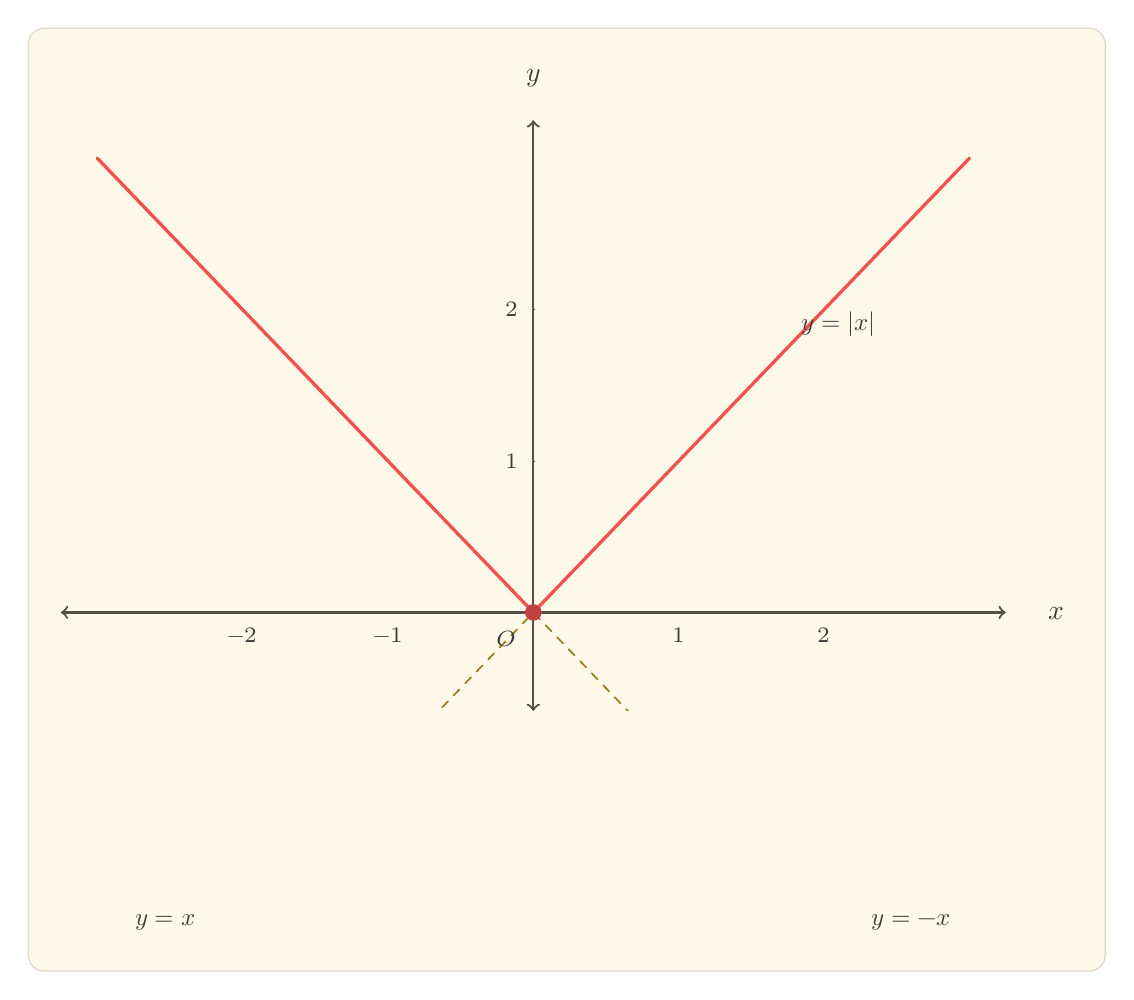
\begin{tikzpicture}[zo graph field]
  \begin{axis}[
    zo axis,
    xmin=-3.25,
    xmax=3.25,
    ymin=-0.65,
    ymax=3.25,
    xtick={-2,-1,1,2},
    ytick={1,2},
    xticklabel=\empty,
    yticklabel=\empty,
    xlabel={$x$},
    ylabel={$y$},
    xlabel style={at={(axis description cs:1.035,0.165)},anchor=west},
    ylabel style={at={(axis description cs:0.5,1.04)},anchor=south}
  ]
    \addplot[zo reference,domain=-3.0:3.0] {x};
    \addplot[zo reference,domain=-3.0:3.0] {-x};

    \addplot[zo graph main,domain=-3.0:0] {-x};
    \addplot[zo graph main,domain=0:3.0] {x};
    \addplot[zo point emphasized] coordinates {(0,0)};

    \node[zo tick label,anchor=north,yshift=-2pt] at (axis cs:-2,0) {$-2$};
    \node[zo tick label,anchor=north,yshift=-2pt] at (axis cs:-1,0) {$-1$};
    \node[zo tick label,anchor=north,yshift=-2pt] at (axis cs:1,0) {$1$};
    \node[zo tick label,anchor=north,yshift=-2pt] at (axis cs:2,0) {$2$};
    \node[zo tick label,anchor=east,xshift=-2pt] at (axis cs:0,1) {$1$};
    \node[zo tick label,anchor=east,xshift=-2pt] at (axis cs:0,2) {$2$};

    \node[zo graph label,anchor=south west,xshift=3pt,yshift=2pt]
      at (axis cs:1.72,1.72) {$y=\lvert x\rvert$};
    \node[zo reference label,anchor=south east,xshift=-3pt,yshift=2pt]
      at (axis cs:-2.2,-2.2) {$y=x$};
    \node[zo reference label,anchor=south west,xshift=3pt,yshift=2pt]
      at (axis cs:2.2,-2.2) {$y=-x$};

    \node[zo tick label,anchor=north east,xshift=-3pt,yshift=-3pt]
      at (axis cs:0,0) {$O$};
  \end{axis}
\end{tikzpicture}
\end{document}
